\documentclass{article}

\PassOptionsToPackage{numbers,compress}{natbib}
\usepackage[preprint]{neurips_2024}

\usepackage[utf8]{inputenc}
\usepackage[T1]{fontenc}
\usepackage{amsmath}
\usepackage{amssymb}
\usepackage{booktabs}
\usepackage{graphicx}
\usepackage{microtype}
\usepackage{xcolor}
\usepackage{hyperref}
\usepackage[capitalize,noabbrev]{cleveref}
\usepackage{enumitem}
\usepackage{balance}
\usepackage{float}
\usepackage{subcaption}
\usepackage{wrapfig}

\definecolor{reportblue}{HTML}{2563EB}
\definecolor{reportred}{HTML}{DC2626}
\definecolor{darkblue}{rgb}{0.10,0.20,0.55}
\hypersetup{
  colorlinks=true,
  citecolor=darkblue,
  linkcolor=darkblue,
  urlcolor=darkblue
}

\setlist[itemize]{leftmargin=*,topsep=2pt,itemsep=1pt,parsep=0pt}
\setlength{\emergencystretch}{1.5em}
\clubpenalty=10000
\widowpenalty=10000
\displaywidowpenalty=10000

\newcommand{\ppl}{\operatorname{PPL}}
\newcommand{\placeholder}[1]{\textcolor{reportred}{\textbf{[#1]}}}

\title{NanoCloud01: Data-Aware Continuation Training\\
for a 99M-Parameter Language Model}

\author{
  Yirui Miao \quad Fengfei Yu \quad Tianyue Zhang \quad Zavier Zhao\\
  CSE 151B/251B, University of California San Diego
}

\begin{document}
\maketitle
\raggedbottom
\setlength{\parfillskip}{0pt plus 0.3\linewidth}

\begin{abstract}
We study autoregressive language modeling under a strict 100M-parameter
limit. We compare three decoder-only designs that allocate capacity across
depth, width, and grouped-query attention (GQA), then continue training the
99.03M-parameter Model~2. All models use RoPE, RMSNorm, SwiGLU, and tied
embeddings. Model~2 is trained on a 50/20/15/15 mixture of FineWeb-Edu,
Wikipedia, science, and books with Muon and AdamW. Its first epoch reaches
21.163 validation perplexity after 38k updates; low-learning-rate
second-epoch continuation reaches \textbf{18.768} at step 69.7k, an 11.3\%
relative reduction. At this scale, data composition, optimizer choice, and
checkpoint selection rival architecture.
\end{abstract}

\section{Introduction}

The NanoGPT competition, based on the compact training framework of
\citet{karpathy2022nanogpt}, asks for next-token prediction over the GPT-2
vocabulary while constraining the submitted model to at most 100M parameters.
For a token sequence $x_{1:T}$, we minimize the following objective:
\begin{equation}
  \mathcal{L}(\theta)
  =-\frac{1}{T}\sum_{t=1}^{T}
  \log p_\theta(x_t\mid x_{<t}),
  \qquad
  \ppl=\exp(\mathcal{L}).
  \label{eq:objective}
\end{equation}
The constraint makes capacity allocation unusually consequential: vocabulary
embeddings already consume a large fraction of the budget, while depth,
attention width, and feed-forward width compete for the remainder. Training
must also generalize across the heterogeneous domains represented by the
provided validation set rather than any single training source.

Our final approach combines a modern compact Transformer with deliberately
balanced data and conservative continuation training. The architecture draws
on rotary position embeddings \citep{su2021roformer}, RMSNorm
\citep{zhang2019root}, SwiGLU \citep{shazeer2020glu}, and grouped-query
attention (GQA) \citep{ainslie2023gqa}. Unlike larger-model work that emphasizes
new modules, our strongest gain comes after the architecture is fixed: a
second epoch resumes the first-epoch checkpoint with progressively smaller
learning rates. Dense evaluation then captures a narrow validation minimum
near convergence during late-stage training.

\paragraph{Contributions.}
First, we compare three sub-100M decoders that trade width and key/value
capacity for depth. Second, we train Model~2 on a reproducible four-source
mixture and show that balanced domains outperform single-source training.
Third, we improve validation perplexity from 21.163 to 18.768 without changing
the model or objective, demonstrating the value of low-rate continuation and
checkpoint selection under a realistic training budget.

\section{Method}

\subsection{Model Family}

All three candidates are pre-normalized decoder-only Transformers with a
1024-token context, GPT-2 BPE, RoPE, RMSNorm, SwiGLU, bias-free projections,
zero dropout, and tied input/output embeddings. They differ in depth, hidden
width, feed-forward width, and key/value sharing; \cref{fig:architecture}
shows the resulting allocations and their depth--sharing trade-off directly.

\begin{figure}[H]
  \centering
  \begin{subfigure}[t]{0.315\linewidth}
    \centering
    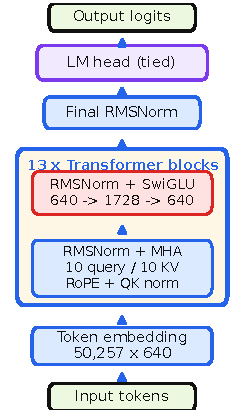
\includegraphics[width=\linewidth]{model1_architecture.pdf}
    \caption{Model~1: 13L, 96.64M.}
  \end{subfigure}\hfill
  \begin{subfigure}[t]{0.315\linewidth}
    \centering
    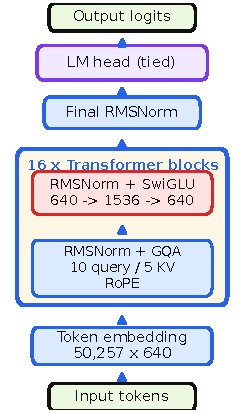
\includegraphics[width=\linewidth]{model2_architecture.pdf}
    \caption{Model~2: 16L, 99.03M.}
  \end{subfigure}\hfill
  \begin{subfigure}[t]{0.315\linewidth}
    \centering
    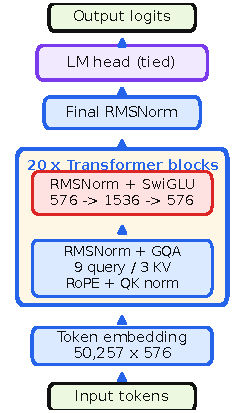
\includegraphics[width=\linewidth]{model3_architecture.pdf}
    \caption{Model~3: 20L, 99.78M.}
  \end{subfigure}
  \caption{Model families under 100M parameters: MHA for Model~1, 1:2 GQA
  for Model~2, and 1:3 GQA for Model~3, enabling progressively greater depth
  under the shared parameter cap.}
  \label{fig:architecture}
\end{figure}

Model~1 uses 13 layers, hidden size 640, 10 query/key/value heads, a
1728-wide MLP, and QK normalization. Model~2 retains width 640 but uses 10
query and 5 key/value heads; the saved attention parameters support 16 layers
with a 1536-wide MLP, totaling 99,032,320 unique parameters. Model~3 is the
deepest design, with 20 layers, width 576, 9 query and 3 key/value heads,
QK normalization, and a 1536-wide MLP. We continue Model~2 because its
complete optimizer, loader, and random-number states were available at the
end of the controlled 38k comparison.

The comparison tests three capacity-allocation strategies. Model~1 spends
more parameters on independent key/value projections, Model~2 uses GQA to
add three layers at the same hidden width, and Model~3 combines stronger GQA
with a narrower residual stream to reach 20 layers. Models~1 and 3 also use
QK normalization, whereas Model~2 does not. Because several dimensions change
together, this is a model-level comparison rather than a component-wise causal
ablation.

\subsection{Data and Optimization}

All sources are tokenized with GPT-2 BPE and stored as \texttt{uint16} binary
arrays or memory-mapped shards. Every training example is a contiguous
1025-token window, split into 1024 inputs and their one-token-shifted targets.
The loader follows an exact 20-example cycle: 10 FineWeb-Edu windows, 4
Wikipedia windows, 3 science windows, and 3 book windows. The cycle is
reshuffled after each pass, while source cursors advance sequentially without
overlap. FineWeb-Edu is the largest source \citep{penedo2024fineweb}; the exact
50/20/15/15 mixture is shown in \cref{tab:ablations}.

Training uses bf16 autocast, gradient clipping at 1.0, micro-batches of 16
sequences, and a global batch of 524,288 tokens per update. We assign
two-dimensional hidden-layer matrices to Muon and embeddings plus remaining
parameters to AdamW, following the small-model training practice popularized
by modded-nanoGPT \citep{jordan2024moddednanogpt}. The first-epoch script
warms up for 200 steps to peak learning rates
$1.3{\times}10^{-2}$ (Muon) and $5.2{\times}10^{-4}$ (AdamW), then cosine
decays to 10\% of each peak by step 38k. It uses only the cross-entropy
objective in \cref{eq:objective}; no teacher or auxiliary loss is present.

The second-epoch script resumes the complete first-epoch state, including
model, optimizer, loader, and random-number states. It keeps the architecture,
data, batch, and objective unchanged, but lowers the effective Muon rate from
approximately
$3.0{\times}10^{-4}$ at step 38k to $3.0{\times}10^{-5}$ near step 69.7k;
the AdamW rate remains 4\% of the Muon rate. We branch from strong
checkpoints at 62k, 63.6k, and 69.6k to shorten each cosine schedule and
evaluate more frequently near convergence.

\section{Experiments}

\subsection{Evaluation Protocol}

We use the course evaluator on \texttt{val.bin}. It computes token-weighted
cross entropy over 1024-token chunks and reports its exponential. Each
evaluation covers 5,169,152 target tokens. The first epoch evaluates every 2k
steps; the second increases frequency from 500 steps to 100 and finally 50
steps. The checkpoint at step 69.7k represents 36.54B sampled training tokens,
of which 19.92B belong to the first epoch. All runs use PyTorch mixed precision
on a single NVIDIA L40S 48GB GPU.

\subsection{Ablations}

\begin{wraptable}{r}{0.45\linewidth}
  \vspace{-0.75\baselineskip}
  \caption{Ablation PPL (lower is better).}
  \label{tab:ablations}
  \centering
  \scriptsize
  \setlength{\tabcolsep}{2.8pt}
  \begin{tabular}{@{}llr@{}}
    \toprule
    Comparison & Setting & PPL \\
    \midrule
    Data source & FineWeb-Edu & 39.67 \\
              & OpenWebText & 65.21 \\
              & 50/20/15/15 mix & \textbf{38.83} \\
    \midrule
    Architecture & Model 1: 13L, MHA & 21.325 \\
                       & Model 2: 16L, GQA 1:2 & 21.163 \\
                       & Model 3: 20L, GQA 1:3 & \textbf{20.918} \\
    \midrule
    Optimizer & AdamW & 39.973 \\
                   & Muon + AdamW & \textbf{36.540} \\
    \bottomrule
  \end{tabular}
\end{wraptable}

\Cref{tab:ablations} isolates data, architecture, and optimization. The
mixture slightly beats FineWeb-Edu and decisively beats OpenWebText. Model~2
improves on Model~1 by 0.162 PPL, while Model~3 gains another 0.245. We
continue Model~2 because its full training state is resumable. Muon + AdamW
lowers PPL from 39.973 to 36.540, an 8.6\% relative gain over AdamW alone in
the controlled optimizer comparison.
For Model~1, raising FineWeb from 50\% to 53\% and 56\% also worsens PPL from
21.325 to 21.460 and 21.609. This supports balanced coverage rather than
increasing FineWeb under the shared comparison budget.

\subsection{Main Result}

\begin{figure}[H]
  \centering
  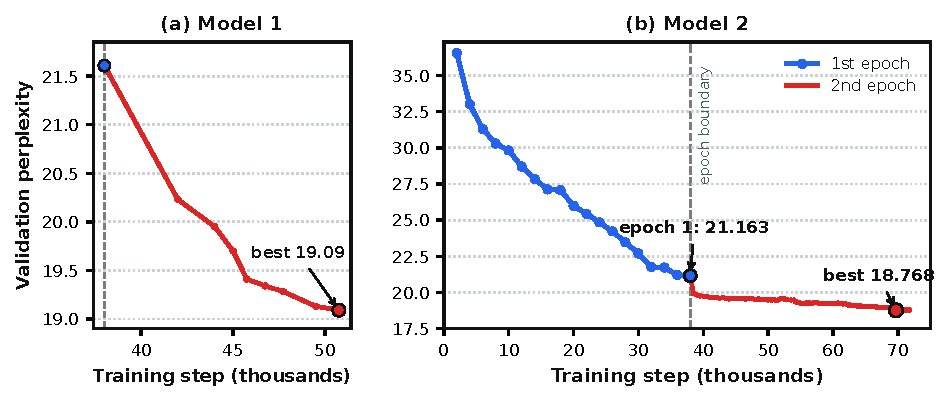
\includegraphics[width=0.98\linewidth]{training_curve.pdf}
  \caption{Low-rate continuation for Models~1 and 2. Red trajectories begin
  at the blue first-epoch endpoints, so each curve is a continuous checkpoint
  lineage. Model~1 values are team-reported; Model~2 values are verified from
  training logs and official evaluations.}
  \label{fig:training}
\end{figure}

\Cref{fig:training} shows consistent continuation gains across architectures.
Model~1 improves from 21.609 to 19.09 by step 50.75k, an 11.7\% relative
reduction. Model~2's first epoch supplies the large representation-learning
gain, reaching 21.163 at 38k; continuation reaches 19.666 at 42k, 19.210 at
62k, and 18.768 at 69.7k. Checkpoints through 71.8k then fluctuate around
18.79--18.81, making dense evaluation part of the method rather than only a
reporting convenience.

The scales of the gains differ substantially. From step 2k to 38k, the first
epoch reduces PPL by 42.1\% relative; continuation then contributes another
11.3\% from the 38k checkpoint. Model~3's 0.245-PPL advantage at 38k is much
smaller than Model~2's 2.395-point continuation gain, although unequal
training budgets prevent a direct ranking after 38k.

The curve also reveals that a single uninterrupted decay is suboptimal near
convergence. Restarting from 62k and 63.6k with smaller schedule scales
recovers steady progress, while the final 69.6k branch resolves a narrow
minimum. These are continuation runs, not separate models: every branch
inherits the same weights, optimizer moments, and data-loader position.

\section{Discussion}

\paragraph{What worked.}
The clearest result is that a fixed 99M architecture still has substantial
headroom after its main schedule. Balanced multi-domain data avoids the severe
failure of OpenWebText-only training, Muon accelerates early optimization, and
low-rate continuation improves the converged checkpoint by 11.3\% relative.
The architecture comparison supports depth over redundant key/value capacity,
but the schedule contributes the largest gain within Model~2.

\paragraph{Interpretation.}
The best 38k architecture is not automatically the best use of total compute.
The model-level ablation favors Model~3 under a matched first-epoch budget,
whereas Model~2 benefits more from a preserved training state and controlled
continuation. Future comparisons should match both sampled tokens and
checkpoint-selection effort, not only parameter count.

\paragraph{Limitations.}
The architecture comparison is not a complete factorial study: Models 1--3
have different depths and GQA ratios, and only Model~2 receives the full
second-epoch continuation budget. Validation-driven branching also risks over-specializing
to \texttt{val.bin}; the final hidden-test result is needed to establish
distributional robustness. Finally, manual branch naming and evaluation
failures at several checkpoints make experiment tracking more fragile than a
single automated sweep.

\paragraph{Next steps.}
Future work should allocate equal token budgets to Models 1--3, automate
best-checkpoint retention, and reserve a second held-out mixture for schedule
selection. A small sweep over source weights around 50/20/15/15 would test
whether the current optimum is robust. Under the same parameter limit,
additional depth should be compared against narrower embeddings using matched
throughput, rather than parameter count alone, in future controlled work.

\paragraph{Team responsibilities.}
Fengfei Yu developed and ran the two-epoch Model~2 training and evaluation
pipeline and consolidated its results.
\placeholder{Team input required: confirm Yirui Miao, Tianyue Zhang, and
Zavier Zhao's responsibilities across Models 1/3, data ablations, slides, and
report writing; also verify final leaderboard and repository details before
submission.}

\paragraph{LLM usage.}
An LLM organized local logs, edited prose, generated plotting code, and
reviewed layout. Claims were checked against source code, evaluation logs,
exported configurations, or the team presentation; the authors remain
responsible for every result, interpretation, final wording, and submitted
artifact carrying their names after independent human review and approval.

\clearpage
\bibliography{references}
\bibliographystyle{plainnat}

\clearpage
\appendix
\section{Reproducibility and Submission Checklist}

\begin{table}[h]
  \centering
  \small
  \caption{Evaluation points used for the ablations in \cref{tab:ablations}.}
  \begin{tabular}{@{}lr@{}}
    \toprule
    Comparison & Training step \\
    \midrule
    Data source & 5,000 \\
    Architecture & 38,000 \\
    Optimizer & 2,000 \\
    Model~1 source-ratio sweep & 38,000 \\
    \bottomrule
  \end{tabular}
\end{table}

\begin{table}[h]
  \centering
  \small
  \begin{tabular}{@{}lp{0.68\textwidth}@{}}
    \toprule
    Item & Location or value \\
    \midrule
    Main training & \path{build-nanogpt/train_gpt2_v13.py} \\
    Continuation & \path{build-nanogpt/train_gpt2_v16.py} \\
    First-epoch checkpoint & \path{build-nanogpt/log/v13/train_ckpt_38000.pt} \\
    Best exported model &
    \path{build-nanogpt/log/v16/.../submission_..._69700} \\
    Best official validation & Step 69,700; PPL 18.7681466; loss 2.932161 nats \\
    Required before submission &
    \placeholder{Add hidden-test PPL/rank, public code/model URLs, and confirmed
    team responsibilities.} \\
    \bottomrule
  \end{tabular}
\end{table}

\end{document}
